
A comparison of force response in the form of normalized lift and drag forces is shown in Figures \ref{fig:lift_zonal_adapt} and \ref{fig:drag_zonal_adapt} respectively. The normalized lift compares well for all the meshes considered. Normalized drag is similar for Mza2 and Mza3 meshes, but shows differences from M0 and Mza1 meshes. Maximum drag in the advancing phases is observed around $\psi=270^\circ$, with Mza3 meshes predicting slightly higher drag than Mza2 meshes, followed by Mza1 and M0 meshes. Major differences in drag between different meshes are observed specifically between phases $\psi=160^\circ$ and $\psi=240^\circ$. Between these phases, Mza2 and Mza3 meshes compare well with each other, whereas M0 and Mza1 meshes predict lower drag than Mza2 and Mza3 meshes. Note that lift and drag response remains unaffected with changes in spanwise resolution for the same in-plane mesh.

\begin{figure}[H]
\centering

\begin{subfigure}[b]{0.7\textwidth}
\centering
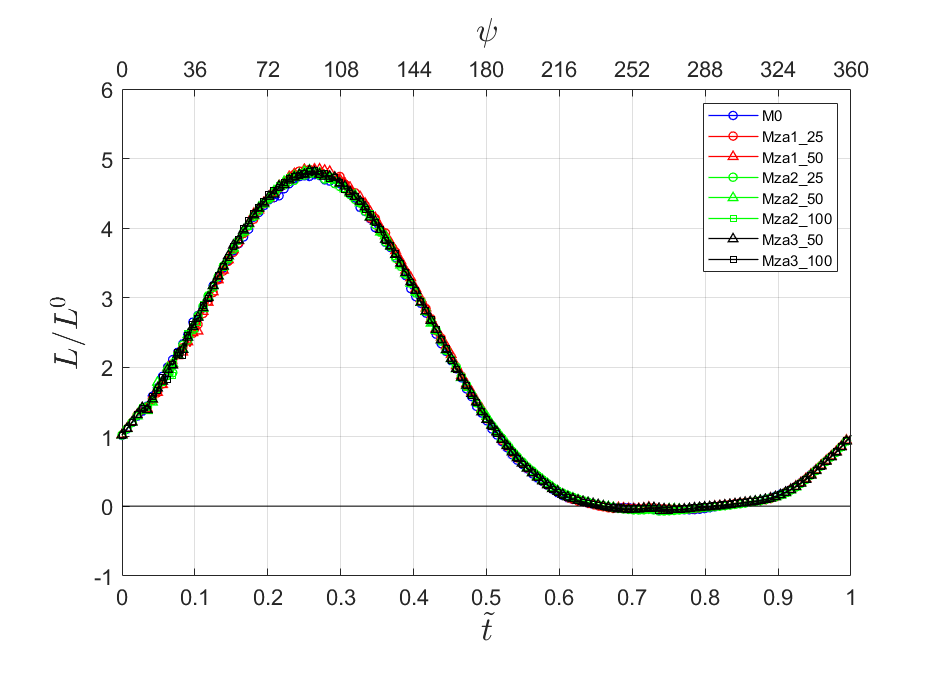
\includegraphics[width=1\textwidth]{figures/zonal_adapt_results/force_response/Lift.png}
\caption{Normalized lift}
\label{fig:lift_zonal_adapt}
\end{subfigure}
\begin{subfigure}[b]{0.7\textwidth}
\centering
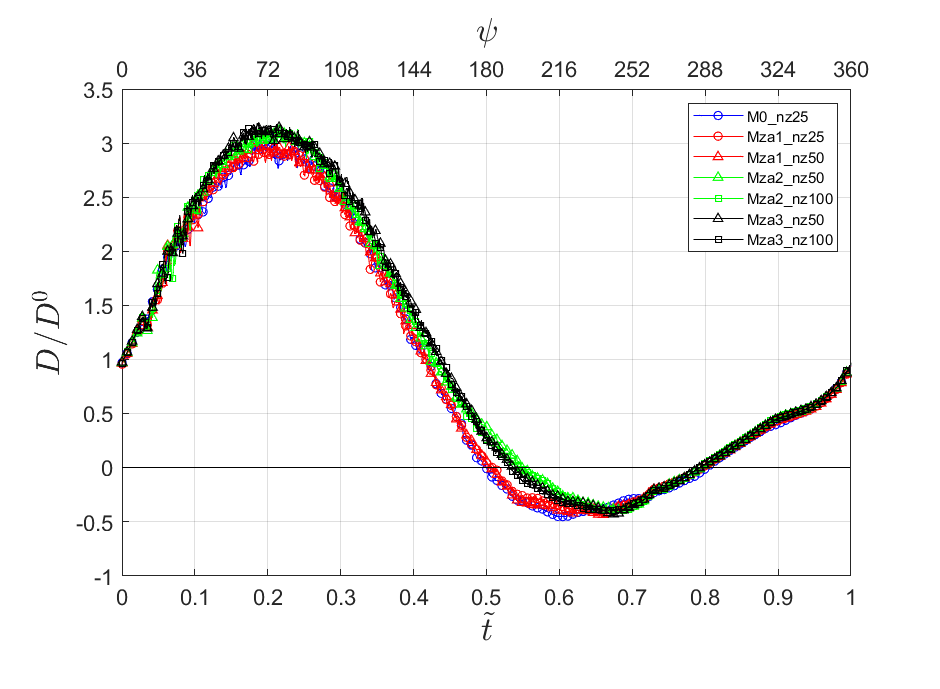
\includegraphics[width=1\textwidth]{figures/zonal_adapt_results/force_response/Drag.png}
\caption{Normalized drag}
\label{fig:drag_zonal_adapt}
\end{subfigure}

\label{fig:force_response_zonal_adapt}
\caption{Normalized forces for different meshes}
\end{figure}